\begin{frame}
  \frametitle{\problemtitle}
  \begin{block}{Problem}
    Spread a number of pizza toppings around a circular pizza such that:
    \begin{itemize}
      \item each pizza topping only appears on some consecutive segment of the slices,
      \item there are at most two toppings on each slice, and
      \item the topping combinations match with a given list of preferences.
    \end{itemize}
  \end{block}
  \vspace{-3mm}
  \begin{center}
    \includegraphics<1>[width=0.23\textwidth]{sample.pdf}
    \includegraphics<2>[width=0.23\textwidth]{sample.pdf}
    \only<2>{\hspace{2cm}}
    \includegraphics<2>[width=0.18\textwidth]{sample-graph.pdf}
  \end{center}
  \only<2>{
    \begin{block}{Insight}
      Model the problem as a graph, with the toppings as nodes and the topping combinations as edges.
    \end{block}
  }
\end{frame}
 \tikzset{
  invisible/.style={opacity=0,text opacity=0},
  onslide/.style={alt={#1{}{invisible}}},
  alt/.code args={<#1>#2#3}{%
    \alt<#1>{\pgfkeysalso{#2}}{\pgfkeysalso{#3}} % \pgfkeysalso doesn't change the path
  },
}
\begin{frame}
  \frametitle{\problemtitle}
  \begin{block}{Solution}
    If any node has at least $3$ non-leaf neighbours, then the answer is \texttt{impossible}:
    \begin{itemize}
      \item<+-> Suppose $1$ has neighbours $2$, $3$ and $4$, which each have a neighbour other than $1$.
      \item<+-> There are slices $(1,2)$, $(1,3)$, $(1,4)$ and $(2,x)$, $(3,y)$, $(4,z)$ with $1 \notin \{x,y,z\}$.
      \item<+-> Place the slices $(1,2)$, $(1,3)$, $(1,4)$ somewhere on the pizza.
      \item<+-> Slices $(2,x)$, $(3,y)$, $(4,z)$ go somewhere between these $\leadsto$ no consecutive range of $1$'s possible.
    \end{itemize}
    \vspace{-3mm}
    \begin{center}
      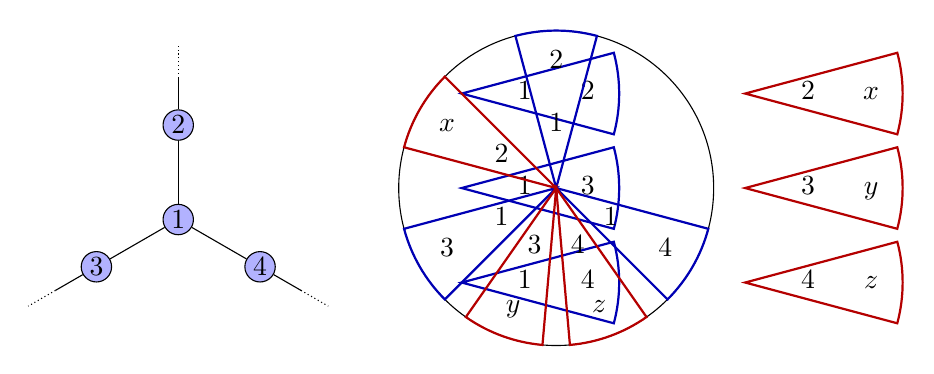
\begin{tikzpicture}[scale=0.4,every node/.style={scale=1,anchor=mid}]
        \definecolor{color1}{RGB}{0,0,180}
        \definecolor{color2}{RGB}{180,0,0}
        \begin{scope}[shift={(-12,-1)},every node/.style={draw,circle,fill=blue!30,minimum size=10,inner sep=1}]
          \node (1) at (0,0) {$1$};
          \node (2) at  (90:3) {$2$};
          \node (3) at (210:3) {$3$};
          \node (4) at (330:3) {$4$};
          \draw (1) -- (2) --  (90:4.5) edge[densely dotted]  (90:5.5);
          \draw (1) -- (3) -- (210:4.5) edge[densely dotted] (210:5.5);
          \draw (1) -- (4) -- (330:4.5) edge[densely dotted] (330:5.5);
        \end{scope}
        \begin{scope}[shift={(-3,3)},onslide=<2>,draw=color1,thick]
          \draw (0,0) -- (-15:5) arc(-15:15:5) -- cycle;
          \node at (0:2) {$1$};
          \node at (0:4) {$2$};
        \end{scope}
        \begin{scope}[shift={(-3,0)},onslide=<2>,draw=color1,thick]
          \draw (0,0) -- (-15:5) arc(-15:15:5) -- cycle;
          \node at (0:2) {$1$};
          \node at (0:4) {$3$};
        \end{scope}
        \begin{scope}[shift={(-3,-3)},onslide=<2>,draw=color1,thick]
          \draw (0,0) -- (-15:5) arc(-15:15:5) -- cycle;
          \node at (0:2) {$1$};
          \node at (0:4) {$4$};
        \end{scope}
        \draw[onslide=<3->] (0,0) circle (5cm);
        \begin{scope}[onslide=<3->,draw=color1,thick]
          \draw (0,0) -- (75:5) arc(75:105:5) -- cycle;
          \draw (0,0) -- (195:5) arc(195:225:5) -- cycle;
          \draw (0,0) -- (315:5) arc(315:345:5) -- cycle;
          \node at (90:2) {$1$};
          \node at (90:4) {$2$};
          \node at (210:2) {$1$};
          \node at (210:4) {$3$};
          \node at (330:2) {$1$};
          \node at (330:4) {$4$};
        \end{scope}
        \begin{scope}[shift={(6,3)},onslide=<2-3>,draw=color2,thick]
          \draw (0,0) -- (-15:5) arc(-15:15:5) -- cycle;
          \node at (0:2) {$2$};
          \node at (0:4) {$x$};
        \end{scope}
        \begin{scope}[shift={(6,0)},onslide=<2-3>,draw=color2,thick]
          \draw (0,0) -- (-15:5) arc(-15:15:5) -- cycle;
          \node at (0:2) {$3$};
          \node at (0:4) {$y$};
        \end{scope}
        \begin{scope}[shift={(6,-3)},onslide=<2-3>,draw=color2,thick]
          \draw (0,0) -- (-15:5) arc(-15:15:5) -- cycle;
          \node at (0:2) {$4$};
          \node at (0:4) {$z$};
        \end{scope}
        \begin{scope}[onslide=<4->,draw=color2,thick]
          \draw (0,0) -- (135:5) arc(135:165:5) -- cycle;
          \draw (0,0) -- (235:5) arc(235:265:5) -- cycle;
          \draw (0,0) -- (275:5) arc(275:305:5) -- cycle;
          \node at (150:2) {$2$};
          \node at (150:4) {$x$};
          \node at (250:2) {$3$};
          \node at (250:4) {$y$};
          \node at (290:2) {$4$};
          \node at (290:4) {$z$};
        \end{scope}
      \end{tikzpicture}
    \end{center}
    \vspace{-2mm}
  \end{block}
\end{frame}
\begin{frame}
  \frametitle{\problemtitle}
  \begin{block}{Solution}
    Otherwise, the graph consists of cycles and paths, possibly with extra leaves and self loops:
    \begin{center}
      \includegraphics[width=0.6\textwidth]{components.pdf}
    \end{center}
    \pause
    \vspace{-4mm}
    \begin{itemize}
      \item<+-> Find all components and determine whether they are cycles or paths, e.g. by counting nodes, edges and loops.
      \item<+-> Remove all degree $0$ vertices, corresponding to toppings not wanted by anybody.
      \item<+-> The answer is \texttt{possible} iff the graph is connected or all components are paths.
      \item<+-> Potential pitfalls: isolated vertices, paths of length $1$, cycles of length $1$, duplicate edges\dots
    \end{itemize}
  \end{block}
  \solvestats
\end{frame}
